\documentclass[a4paper, 12pt]{article}
\usepackage{graphicx}
\graphicspath{ {../images/} }
% Title information
\title{Réseaux : notes de cours}
\author{Arian Dervishaj}
\date{\today}

\begin{document}
\maketitle
\pagebreak

\subsection*{Protocole d'application}
\begin{itemize}
    \item URL \begin{itemize}
        \item Localisateur de ressources uniforme
        \item http://www.cs.princeton.edu/~llp/index.html
    \end{itemize}
    \item HTTP \begin{itemize}
        \item Protocole de transfert hypertexte
    \end{itemize}
    \item TCP \begin{itemize}
        \item Protocole de controle de transmission
    \end{itemize}
    \item 17 messages pour une demande d'URL \begin{itemize}
        \item 6 pour trouver l'adresse IP
        \item 3 pour l'établissement de la connexion TCP4 pour la requete HTTP et l'accusé de reception
        \item 4 messages pour supprimer la connexion TCP
    \end{itemize}
\end{itemize}

\subsection*{Topologie réseau}
\begin{minipage}{0.3\textwidth}
    \begin{itemize}
        \item Point à point
        \item Bus
        \item Ring
        \item Star
        \item Full mesh
        \item Étoile étendue
        \item Distribué
    \end{itemize}
\end{minipage}
\begin{minipage}{0.6\textwidth}
    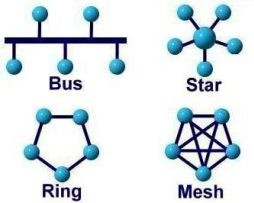
\includegraphics{topologie.jpeg}
\end{minipage}

\subsection*{}
\textbf{Definition récursive d'un réseau :} 
Un réseau informatique est un système constitué d'au moins deux nœuds connectés, construit en imbriquant des réseaux à des niveaux d'abstraction de plus en plus bas, avec une infrastructure physique sous-jacente.


\end{document}
